\documentclass[a4paper,10pt]{article}
\usepackage[margin=1in]{geometry}
\usepackage{polski}
\usepackage[utf8x]{inputenc}
\usepackage[unicode]{hyperref}
\usepackage{amssymb}
\usepackage{xifthen}
\usepackage[fleqn]{amsmath}
\usepackage{todonotes}
\usepackage{graphicx}
\usepackage{float}
\usepackage{fullpage}
\usepackage{epstopdf}
\usepackage{multirow}
\usepackage{subfig}
\usepackage[europeanresistors,americaninductors]{circuitikz}
\usetikzlibrary{patterns}
\newcommand{\withtodo}{0}


\def\arraystretch{1}


\begin{document}

\begin{table}
  \centering
  \def\arraystretch{1.5}
    \begin{tabular}{ l l l l } \hline
    Wydział:           & \multicolumn{2}{l }{Dzień:Poniedziałek 14-17}    &Zespół:  \\
    Fizyki             &    \multicolumn{2}{l }{Data: 20.03.2017}         &8             \\\hline
    Imiona i nazwiska: &Ocena z przygotowania:  &Ocena ze sprawozdania:   &Ocena końcowa: \\
    Marta Pogorzelska  &                        &                         &                \\
    Paulina Marikin    &                        &                         &\\\hline
    \multicolumn{2}{ l }{Prowadzący:                 } &\multicolumn{2}{l }{Podpis:             }  \\\hline
  \end{tabular}
\end{table}

\title{Ćwiczenie 45:\\Stany wzbudzenia atomów rtęci i neonu\\Badanie efektu Franca-Hertza}
\date{}
\maketitle
\section{Wstęp teoretyczny}
Poziomy energetyczne elektronów w atomie są skwantowane, czyli mogą przyjmować tylko określone, dyskretne wartości. Zmiana poziomu energetycznego
z niższego na wyższy (wzbudzony) może zajść tylko wtedy, gdy elektron otrzyma ilość energii równą różnicy między tymi poziomami. James Franc i Gustaw
Hertz w swoim doświadczeniu z 1913 roku potwierdzili ten fakt, czym pomogli ugruntować kwantową teorię atomu. W swoim eksperymencie badali
przewodzenie prądu przez elektrony w lampach wypełnionych gazowym neonem albo oparami rtęci. Zmiana prądu anodowego związana ze zwiększaniem
energii dostarczanej do elektronów nie zachodzi w takim przypadku monotonicznie, ale rośnie i maleje w równych przedziałach czasu. Dzieje się tak,
gdyż atomy mogą pochłaniać energie rozpędzonych elektronów dopiero, gdy osiągnie ona konkretną wartość odpowiadającą różnicy między dwoma poziomami
energetycznymi.

\section{Opis układu i metody pomiarowej}
W skład układu pomiarowego dla lampy rtęciowej wchodzą:
\begin{itemize}
  \item lampa rtęciowa
  \item piec do ogrzania rtęci
  \item termopara z woltomierzem mierząca temperaturę rtęci
  \item wentylator
  \item zasilacz umożliwiający regulację napięcia żarzenia, napięcia hamowania i napięcia przyspieszającego
  \item 4 woltomierze mierzące powyższe napięcia i napięcie anodowe
\end{itemize}
Układ pomiarowy dla neonu jest podobny, jednak nie zawiera pieca, termopary ani wentylatora, gdyż neon w temperaturze pokojowej jest w stanie gazowym. Zawiera zaś niewystępującą w
zestawie rtęci siatkę pozwalającą na ukierunkowanie strumienia elektronów.\\
W dowiadczeniu najpierw podgrzano rtęć do postaci gazowej. Następnie ustalono, stałe przez całe doświadczenie, napięcie żarzenia i napięcie hamowania. Mierzone było napięcie
anodowe (będące wprost proporcjonalne do prądu anodowego) w zależności o zmienianego przez eksperymentatora napięcia przyspieszającego w zakresie od 0 do 30 voltów. Doświadczenie
dla neonu przebiegało analogicznie. Jedynymi różnicami był brak początkowego podgrzewania i zakres napięcia przyspieszającego od 0 do 70 voltów.

\section{Wyniki pomiarów}
\subsection{Rtęć}
\begin{figure}[H]
\begin{tabular}{lrrrrrrrrrrrrr}
{} &    0  &    1  &    2  &    3  &    4  &    5  &    6  &    7  &    8  &    9  &    10 &    11 &    12 \\
U[V]  &  0.20 &  0.50 &  2.60 &  3.60 &  4.50 &  5.50 &  6.60 &  7.60 &  8.20 &  9.00 &  9.40 &  10.6 &  11.0 \\
Ua[mV] &  3.12 &  3.18 &  3.82 &  3.01 &  2.85 &  3.75 &  4.26 &  4.11 &  3.69 &  4.15 &  4.85 &  10.6 &  12.1 \\
\end{tabular}
\end{figure}

\begin{figure}[H]
\begin{tabular}{l rrrrrrrrrrrr}
{} &     14 &     15 &     16 &     17 &     18 &     19 &     20 &    21 &    22 &     23 &     24 &     25 \\
U[V]  &  11.60 &  12.50 &  13.10 &  13.30 &  13.50 &  14.20 &  15.20 &  15.7 &  16.2 &  16.40 &  16.60 &  17.60 \\
Ua[mV] &  13.18 &   6.42 &   4.59 &   4.31 &   4.65 &   5.69 &  11.26 &  16.6 &  19.7 &  19.89 &  18.22 &   7.65 \\
\end{tabular}
\end{figure}

\begin{figure}[H]
\begin{tabular}{l rrrrrrrrrrrr}
{} &     27 &     28 &     29 &     30 &     31 &     32 &     33 &    34 &     35 &    36 &     37 &     38 \\
U[V]  &  18.30 &  18.90 &  20.00 &  20.50 &  20.80 &  21.10 &  21.40 &  21.7 &  22.70 &  23.2 &  23.50 &  23.90 \\
Ua[mV] &   5.17 &   5.87 &  12.68 &  18.78 &  23.37 &  26.53 &  27.97 &  26.7 &  12.85 &   9.5 &   8.41 &   9.06 \\
\end{tabular}
\end{figure}

\begin{figure}[H]
\begin{tabular}{l rrrrrrrrrrr}
{} &     40 &     41 &     42 &     43 &     44 &     45 &     46 &     47 &     48 &     49 &     50 \\
U[V]  &  25.10 &  26.10 &  26.40 &  26.80 &  27.20 &  28.20 &  28.60 &  29.20 &  29.50 &  30.50 &  30.90 \\
Ua[mV] &  19.38 &  32.45 &  34.67 &  34.68 &  31.35 &  19.44 &  17.12 &  16.76 &  18.05 &  28.12 &  33.55 \\
\end{tabular}
\end{figure}
\subsection{Neon}
\begin{figure}[H]
\begin{tabular}{lrrrrrrrrrrrr}
{} &    0  &    1  &    2  &    3  &    4  &    5  &    6  &    7  &    8  &     9  &     10 &     11 \\
U[V]  &  0.00 &  1.10 &  2.30 &  3.50 &  5.10 &  6.00 &  7.40 &  8.80 &  9.70 &  10.60 &  11.30 &  12.40 \\
Ua[mV] &  0.86 &  0.85 &  0.97 &  0.85 &  1.06 &  1.45 &  1.86 &  2.13 &  2.33 &   2.55 &   2.63 &   2.84 \\
\end{tabular}
\end{figure}
\begin{figure}[H]
\begin{tabular}{lrrrrrrrrrrr}
{} &     13 &     14 &     15 &     16 &     17 &     18 &     19 &     20 &     21 &     22 &     23 \\
U[V]  &  14.90 &  15.80 &  16.80 &  18.10 &  20.30 &  20.90 &  21.50 &  22.00 &  22.70 &  23.70 &  25.00 \\
Ua[mV] &   3.23 &   3.41 &   3.51 &   3.12 &   1.67 &   1.57 &   1.42 &   1.23 &   1.72 &   3.42 &   6.11 \\
\end{tabular}
\end{figure}

\begin{figure}[H]
\begin{tabular}{lrrrrrrrrrrr}

{} &     25 &     26 &     27 &    28 &     29 &     30 &     31 &     32 &     33 &     34 &     35 \\

U[V]  &  26.00 &  28.00 &  28.50 &  29.1 &  30.00 &  31.10 &  32.60 &  33.70 &  34.50 &  36.60 &  37.50 \\
Ua[mV] &   7.76 &  10.03 &  10.44 &  10.8 &  11.07 &  11.78 &  12.37 &  12.69 &  11.42 &   5.56 &   3.34 \\

\end{tabular}
\end{figure}

\begin{figure}[H]
\begin{tabular}{lrrrrrrrrrrr}

{} &     37 &    38 &     39 &     40 &     41 &     42 &     43 &     44 &     45 &     46 &     47 \\

U[V]  &  39.50 &  40.6 &  42.30 &  43.30 &  44.30 &  45.30 &  46.50 &  47.00 &  47.50 &  48.00 &  49.00 \\
Ua[mV] &   2.04 &   4.9 &  10.09 &  12.71 &  14.85 &  16.33 &  17.88 &  18.27 &  18.77 &  19.27 &  19.96 \\

\end{tabular}
\end{figure}

\begin{figure}[H]
\begin{tabular}{lrrrrrrrrrrr}

{} &     49 &     50 &     51 &     52 &     53 &     54 &     55 &     56 &     57 &     58 &     59 \\

U[V]  &  50.00 &  51.00 &  51.50 &  54.00 &  56.00 &  56.50 &  57.00 &  57.50 &  60.00 &  63.00 &  64.10 \\
Ua[mV] &  20.52 &  20.49 &  19.58 &  11.11 &   5.55 &   5.53 &   6.43 &   7.48 &  14.01 &  22.51 &  24.77 \\

\end{tabular}
\end{figure}

\begin{figure}[H]
\begin{tabular}{lrrrrrr}

{} &     61 &     62 &     63 &     64 &     65 &     66 \\

U[V]  &  66.00 &  66.60 &  67.10 &  67.60 &  68.10 &  68.60 \\
Ua[mV] &  28.18 &  29.21 &  29.76 &  30.31 &  30.14 &  29.61 \\

\end{tabular}
\end{figure}
\section{Analiza wyników}
Uzyskane wyniki napięcia anodowego przeskalowano przez czynnik : $10^8 \frac{V}{A}$ w celu uzyskania prądu anodowego. Następnie otrzymane wyniki wraz z niepewnościami przedstawiono na wykresie, z którego odczytano kolejne ekstrema.
\begin{figure} [H]
    \centering
  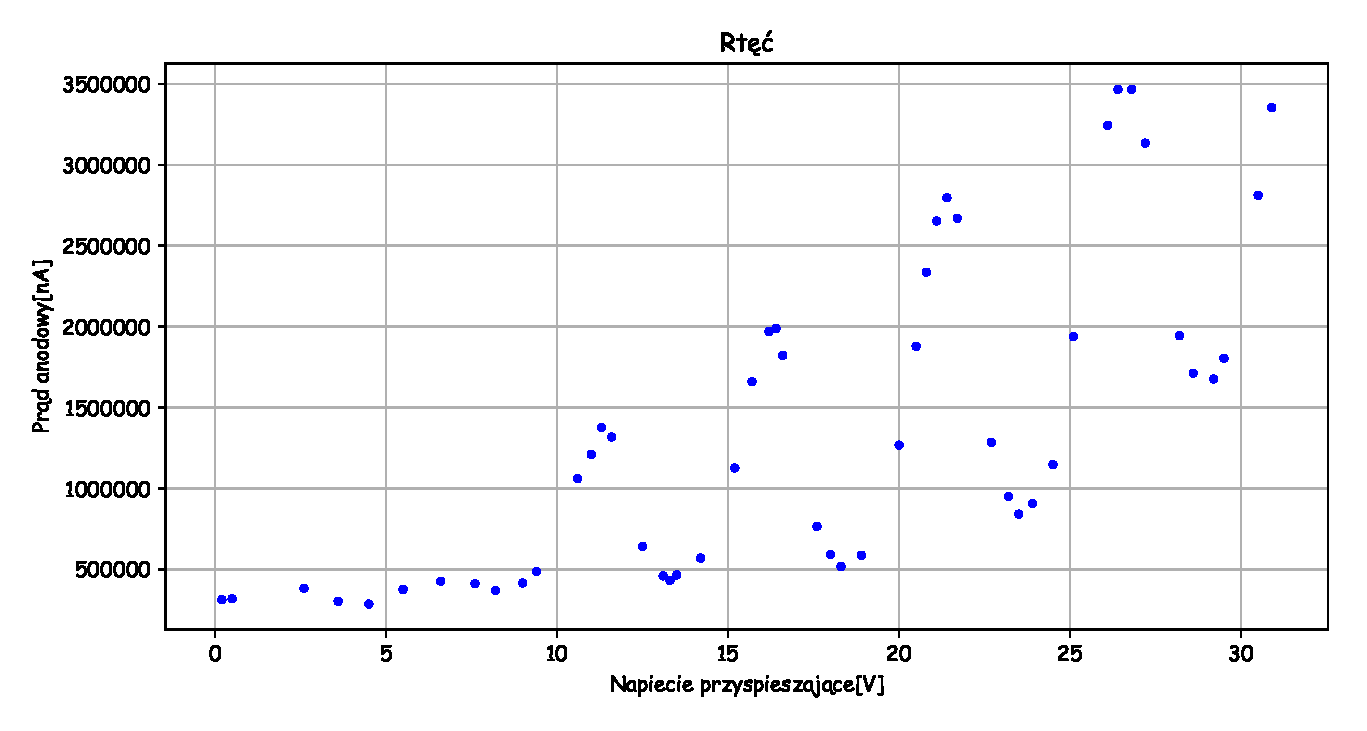
\includegraphics[width=\textwidth]{./rtec.eps}
  %\caption{}
  \label{}
\end{figure}
\begin{tabular}{cc|cc}
  \multicolumn{2}{l |}{Minimum}&\multicolumn{2}{l }{Maksimum}\\
  U[V] & I[nA] & U[V] & I[nA] \\
  4.5  & 28.5  & 6.6  & 42.6  \\
  8.2  & 36.9  & 11.3 & 137.7 \\
  14.3 & 43.1  & 16.4 & 198.9 \\
  18.3 & 51.7  & 21.4 & 279.7 \\
  23.5 & 84.1  & 26.4 & 346.8 \\
  29.2 & 167.6 && \\
\end{tabular}
\begin{figure} [H]
    \centering
  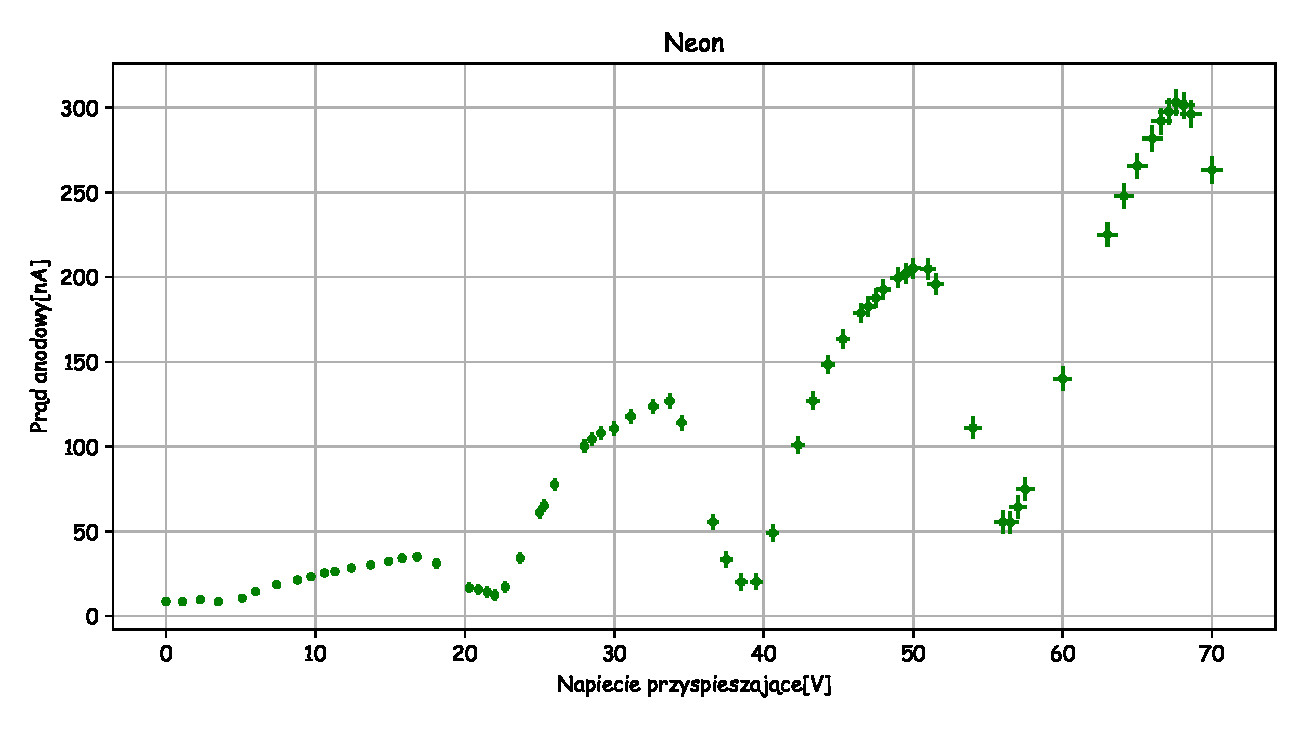
\includegraphics[width=\textwidth]{./neon.eps}
  %\caption{}
  \label{}
\end{figure}
\begin{tabular}{cc|cc}
  \multicolumn{2}{l |}{Minimum}&\multicolumn{2}{l }{Maksimum}\\
  U[V] & I[nA]& U[V] & I[nA] \\
  22.0 & 12.3 & 16.8 & 35.8 \\
  38.5 & 20.2 & 33.7 & 126.9 \\
  56.5 & 55.3 & 50.0 & 205.2 \\
       &      & 67.6 & 303.1 \\
\end{tabular}

Z uzyskanych wynikow można wyliczyć różnicę napięć miedzy kolejnymi maksimami/minimami i, przemnażając ją przez $e = 1.602*10^{-19}C$, energię wzbudzenia.
\\\\
\begin{tabular}{|l|cc|cc|}
\hline
{} &  \multicolumn{2}{c |}{Rtęc}&\multicolumn{2}{c |}{Neon}\\\hline
{} & Z minimow & Z maksimow & Z minimow & Z maksimow \\\hline
rożnica napiec[V]& 4.94(6)& 5.05(7) & 17.25(30) & 16.93(23) \\\hline
energia wzbudzenia[eV]& 4.94(6)& 5.05(7) & 17.25(30) & 16.93(23)\\\hline
\end{tabular}

\section{Analiza niepewności}
Niepewności pomiarów zostały wyliczone ze wzoru:
\begin{equation}
  \Delta U = U*klasa + 1*rozdzielczosc
\end{equation}
,gdzie klasa używanego woltomierza wynosi 0.01, zaś za rozdzielczość przyjęto najmniejsze możliwe wskazanie woltomierza w danym ustawieniu.
\\
W celu otrzymania niepewności prądu anodowego przeskalowano niepewność odpowiadającego mu napięcia anodowego przez ten sam czynnik skalujący co wcześniej same napięcia.
Wreszcie, niepewności różnic napięć wyliczono metodą propagacji niepewności:
\begin{equation}
  \Delta U_{między} = \sqrt{\Delta U_n^2+\Delta U_1^2} \frac{1}{n-1}
\end{equation}

\section{Wnioski}
Otrzymane wyniki dla maksimów i minimów są zgodne w dwóch przedziałach niepewności. Wartosci dla rtęci są także zgodne z wynikami uzyskanymi przez Franca i Hertza w 1913r: 4.9V. Wyniki dla neonu są nieco poniżej tablicowego 18.7V, jednak ogólny kształt wykresu został zachowany. W obu przypadkach wartości wyliczone z minimów są bliższe tablicowym.  
\end{document}
